% -*- coding: utf-8 -*-
%\documentclass[output=paper]{LSP/langsci} 
\documentclass[output=paper
,newtxmath
,modfonts
,nonflat]{langsci/langscibook} 
% \bibliography{localbibliography} 
% \usepackage{pifont}
\usepackage{savesym}

\savesymbol{downingtriple}
\savesymbol{downingdouble}
\savesymbol{downingquad}
\savesymbol{downingquint}
\savesymbol{suph}
\savesymbol{supj}
\savesymbol{supw}
\savesymbol{sups}
\savesymbol{ts}
\savesymbol{tS}
\savesymbol{devi}
\savesymbol{devu}
\savesymbol{devy}
\savesymbol{deva}
\savesymbol{N}
\savesymbol{Z}
\savesymbol{circled}
\savesymbol{sem}
\savesymbol{row}
\savesymbol{tipa}
\savesymbol{tableauxcounter}
\savesymbol{tabhead}
\savesymbol{inp}
\savesymbol{inpno}
\savesymbol{g}
\savesymbol{hanl}
\savesymbol{hanr}
\savesymbol{kuku}
\savesymbol{ip}
\savesymbol{lipm}
\savesymbol{ripm}
\savesymbol{lipn}
\savesymbol{ripn} 
% \usepackage{amsmath} 
% \usepackage{multicol}
\usepackage{qtree} 
\usepackage{tikz-qtree,tikz-qtree-compat}
% \usepackage{tikz}
\usepackage{upgreek}


%%%%%%%%%%%%%%%%%%%%%%%%%%%%%%%%%%%%%%%%%%%%%%%%%%%%
%%%                                              %%%
%%%           Examples                           %%%
%%%                                              %%%
%%%%%%%%%%%%%%%%%%%%%%%%%%%%%%%%%%%%%%%%%%%%%%%%%%%%
% remove the percentage signs in the following lines
% if your book makes use of linguistic examples
\usepackage{tipa}  
\usepackage{pstricks,pst-xkey,pst-asr}

%for sande et al
\usepackage{pst-jtree}
\usepackage{pst-node}
%\usepackage{savesym}


% \usepackage{subcaption}
\usepackage{multirow}  
\usepackage{./langsci/styles/langsci-optional} 
\usepackage{./langsci/styles/langsci-lgr} 
\usepackage{./langsci/styles/langsci-glyphs} 
\usepackage[normalem]{ulem}
%% if you want the source line of examples to be in italics, uncomment the following line
% \def\exfont{\it}
\usetikzlibrary{arrows.meta,topaths,trees}
\usepackage[linguistics]{forest}
\forestset{
	fairly nice empty nodes/.style={
		delay={where content={}{shape=coordinate,for parent={
					for children={anchor=north}}}{}}
}}
\usepackage{soul}
\usepackage{arydshln}
% \usepackage{subfloat}
\usepackage{langsci/styles/langsci-gb4e} 
   
% \usepackage{linguex}
\usepackage{vowel}

\usepackage{pifont}% http://ctan.org/pkg/pifont
\newcommand{\cmark}{\ding{51}}%
\newcommand{\xmark}{\ding{55}}%
 
 
 %Lamont
 \makeatletter
\g@addto@macro\@floatboxreset\centering
\makeatother

\usepackage{newfloat} 
\DeclareFloatingEnvironment[fileext=tbx,name=Tableau]{tableau}
% %% hyphenation points for line breaks
%% Normally, automatic hyphenation in LaTeX is very good
%% If a word is mis-hyphenated, add it to this file
%%
%% add information to TeX file before \begin{document} with:
%% %% hyphenation points for line breaks
%% Normally, automatic hyphenation in LaTeX is very good
%% If a word is mis-hyphenated, add it to this file
%%
%% add information to TeX file before \begin{document} with:
%% %% hyphenation points for line breaks
%% Normally, automatic hyphenation in LaTeX is very good
%% If a word is mis-hyphenated, add it to this file
%%
%% add information to TeX file before \begin{document} with:
%% \include{localhyphenation}
\hyphenation{
affri-ca-te
affri-ca-tes
com-ple-ments
par-a-digm
Sha-ron
Kings-ton
phe-nom-e-non
Daul-ton
Abu-ba-ka-ri
Ngo-nya-ni
Clem-ents 
King-ston
Tru-cken-brodt
Tab-leau
cophono-logies
mark-edness
Ti-gri-nya
a-mong
Car-stens
Lu-bu-ku-su
}
\hyphenation{
affri-ca-te
affri-ca-tes
com-ple-ments
par-a-digm
Sha-ron
Kings-ton
phe-nom-e-non
Daul-ton
Abu-ba-ka-ri
Ngo-nya-ni
Clem-ents 
King-ston
Tru-cken-brodt
Tab-leau
cophono-logies
mark-edness
Ti-gri-nya
a-mong
Car-stens
Lu-bu-ku-su
}
\hyphenation{
affri-ca-te
affri-ca-tes
com-ple-ments
par-a-digm
Sha-ron
Kings-ton
phe-nom-e-non
Daul-ton
Abu-ba-ka-ri
Ngo-nya-ni
Clem-ents 
King-ston
Tru-cken-brodt
Tab-leau
cophono-logies
mark-edness
Ti-gri-nya
a-mong
Car-stens
Lu-bu-ku-su
}
% %add all your local new commands to this file
\newcommand{\downingquad}[4]{\parbox{2.5cm}{#1}\parbox{3.5cm}{#2}\parbox{2.5cm}{#3}\parbox{3.5cm}{#4}}
\newcommand{\downingtriple}[3]{\parbox{4.5cm}{#1}\parbox{3cm}{#2}\parbox{3cm}{#3}}
\newcommand{\downingdouble}[2]{\parbox{4.5cm}{#1}\parbox{6cm}{#2}}
\newcommand{\downingquint}[5]{\parbox{1.75cm}{#1}\parbox{2.25cm}{#2}\parbox{2cm}{#3}\parbox{3cm}{#4}\parbox{2cm}{#5}}
\newcolumntype{Y}{>{\centering\arraybackslash}X}
\newcolumntype{T}{>{\centering\arraybackslash}m{2cm}}

%commands for Kusmer paper below
\newcommand{\ip}{$\upiota$}
\newcommand{\lipm}{(\_{\ip-Max}}
\newcommand{\ripm}{)\_{\ip-Max}}
\newcommand{\lipn}{(\_{\ip}}
\newcommand{\ripn}{)\_{\ip}}
\renewcommand{\_}[1]{\textsubscript{#1}}


%commands for Pillion paper below
\newcommand{\suph}{\textipa{\super h}}
\newcommand{\supj}{\textipa{\super j}}
\newcommand{\supw}{\textipa{\super w}}
\newcommand{\ts}{\textipa{\t{ts}}}
\newcommand{\tS}{\textipa{\t{tS}}}
\newcommand{\devi}{\textipa{\r*i}}
\newcommand{\devu}{\textipa{\r*u}}
\newcommand{\devy}{\textipa{\r*y}}
\newcommand{\deva}{\textipa{\r*a}}
\renewcommand{\N}{\textipa{N}}
\newcommand{\Z}{\textipa{Z}}
% 

%commands for Diercks paper below
\newcommand{\circled}[1]{\begin{tikzpicture}[baseline=(word.base)]
\node[draw, rounded corners, text height=8pt, text depth=2pt, inner sep=2pt, outer sep=0pt, use as bounding box] (word) {#1};
\end{tikzpicture}
}

%commands for Pesetsky paper below
% \newcommand{\sem}[2][]{\mbox{$[\![ $\textbf{#2}$ ]\!]^{#1}$}}
\newcommand{\sem}[2][]{\mbox{$[[ $\textbf{#2}$ ]]^{#1}$}}

% \newcommand{\ripn}{{\color{red}ripn}}%this is used but never defined. Please update the definition



%commands for Lamont paper below
\newcommand{\row}[4]{
	#1. & 
    /{#2}/ & 
    [{#3}] & 
    `#4' \\ 
}
%\newcounter{tableauxcounter}
\newcommand{\tabhead}[2]{
%     \captionsetup{labelformat=empty}
%     \stepcounter{tableauxcounter}
%     \addtocounter{table}{-1}
% 	\centering
% 	\caption{Tableau \thetableauxcounter: #1}
	\caption{#1}
	\label{#2}
}
\newcommand{\candref}[2]{{(\ref{#1}#2)}}
\newcommand{\tableauref}[1]{{Tableau~\ref{#1}}}
% tableaux
\newcommand{\inp}[1]{\multicolumn{2}{|l||}{{#1}}}
\newcommand{\inpno}[1]{\multicolumn{2}{|l||}{#1}}
\newcommand{\g}{\cellcolor{lightgray}}
\newcommand{\hanl}{\HandLeft}
\newcommand{\hanr}{\HandRight}
\newcommand{\kuku}{Kuk\'{u}}

% \newcommand{\nocaption}[1]{{\color{red} Please provide a caption}}

% \providecommand{\biberror}[1]{{\color{red}#1}}

\definecolor{RED}{cmyk}{0.05,1,0.8,0}


\newfontfamily\amharicfont[Script = Ethiopic, Scale = 1.0]{AbyssinicaSIL}
\newcommand{\amh}[1]{{\amharicfont #1}}

% 
% %Gjersoe
\usepackage{textgreek}
% 
\newcommand{\viol}{\fontfamily{MinionPro-OsF}\selectfont\rotatebox{60}{$\star$}}
\newcommand{\myscalex}{0.45}
\newcommand{\myscaley}{0.65}
%\newcommand{\red}[1]{\textcolor{red}{#1}}
%\newcommand{\blue}[1]{\textcolor{blue}{#1}}
\newcommand{\epen}[1]{\colorbox{jgray}{#1}}
\newcommand{\hand}{{\normalsize \ding{43}}}
\definecolor{jgray}{gray}{0.8} 
\usetikzlibrary{positioning}
\usetikzlibrary{matrix}
\newcommand{\mora}{\textmu\xspace}
\newcommand{\si}{\textsigma\xspace}
\newcommand{\ft}{\textPhi\xspace}
\newcommand{\tone}{\texttau\xspace}
\newcommand{\word}{\textomega\xspace}
% \newcommand{\ts}{\texttslig}
\newcommand{\fns}{\footnotesize}
\newcommand{\ns}{\normalsize}
\newcommand{\vs}{\vspace{1em}}
\newcommand{\bs}{\textbackslash}   % backslash
\newcommand{\cmd}[1]{{\bf \color{red}#1}}   % highlights command
\newcommand{\scell}[2][l]{\begin{tabular}[#1]{@{}c@{}}#2\end{tabular}}
% \interfootnotelinepenalty=10000

% --- Snider Representations --- %

\newcommand{\RepLevelHh}{
\begin{minipage}{0.10\textwidth}
\begin{tikzpicture}[xscale=\myscalex,yscale=\myscaley]
%\node (syl) at (0,0) {Hi};
\node (Rt) at (0,1) {o};
\node (H) at (-0.5,2) {H};
\node (R) at (0.5,3) {h};
%\draw [thick] (syl.north) -- (Rt.south) ;
\draw [thick] (Rt.north) -- (H.south) ;
\draw [thick] (Rt.north) -- (R.south) ;
\end{tikzpicture}
\end{minipage}
}

\newcommand{\RepLevelLh}{
\begin{minipage}{0.10\textwidth}
\begin{tikzpicture}[xscale=\myscalex,yscale=\myscaley]
%\node (syl) at (0,0) {Mid2};
\node (Rt) at (0,1) {o};
\node (H) at (-0.5,2) {L};
\node (R) at (0.5,3) {h};
%\draw [thick] (syl.north) -- (Rt.south) ;
\draw [thick] (Rt.north) -- (H.south) ;
\draw [thick] (Rt.north) -- (R.south) ;
\end{tikzpicture}
\end{minipage}
}

\newcommand{\RepLevelHl}{
\begin{minipage}{0.10\textwidth}
\begin{tikzpicture}[xscale=\myscalex,yscale=\myscaley]
%\node (syl) at (0,0) {Mid1};
\node (Rt) at (0,1) {o};
\node (H) at (-0.5,2) {H};
\node (R) at (0.5,3) {l};
%\draw [thick] (syl.north) -- (Rt.south) ;
\draw [thick] (Rt.north) -- (H.south) ;
\draw [thick] (Rt.north) -- (R.south) ;
\end{tikzpicture}
\end{minipage}
}

\newcommand{\RepLevelLl}{
\begin{minipage}{0.10\textwidth}
\begin{tikzpicture}[xscale=\myscalex,yscale=\myscaley]
%\node (syl) at (0,0) {Lo};
\node (Rt) at (0,1) {o};
\node (H) at (-0.5,2) {L};
\node (R) at (0.5,3) {l};
%\draw [thick] (syl.north) -- (Rt.south) ;
\draw [thick] (Rt.north) -- (H.south) ;
\draw [thick] (Rt.north) -- (R.south) ;
\end{tikzpicture}
\end{minipage}
}

% --- Representations --- %

\newcommand{\RepLevel}{
\begin{minipage}{0.10\textwidth}
\begin{tikzpicture}[xscale=\myscalex,yscale=\myscaley]
\node (syl) at (0,0) {\textsigma};
\node (Rt) at (0,1) {o};
\node (H) at (-0.5,2) {\texttau};
\node (R) at (0.5,3) {\textrho};
\draw [thick] (syl.north) -- (Rt.south) ;
\draw [thick] (Rt.north) -- (H.south) ;
\draw [thick] (Rt.north) -- (R.south) ;
\end{tikzpicture}
\end{minipage}
}

\newcommand{\RepContour}{
\begin{minipage}{0.10\textwidth}
\begin{tikzpicture}[xscale=\myscalex,yscale=\myscaley]
\node (syl) at (0,0) {\textsigma};
\node (Rt) at (0,1) {o};
\node (H) at (-0.5,2) {\texttau};
\node (R) at (0.5,3) {\textrho};
\node (Rt2) at (1.5,1.0) {o};
%\node (H2) at (1.0,2) {$\tau$};
%\node (R2) at (2.0,2.5) {R};
\draw [thick] (syl.north) -- (Rt.south) ;
\draw [thick] (Rt.north) -- (H.south) ;
\draw [thick] (Rt.north) -- (R.south) ;
\draw [thick] (syl.north) -- (Rt2.south) ;
%\draw [thick] (Rt2.north) -- (H2.south) ;
%\draw [thick] (Rt2.north) -- (R2.south) ;
\end{tikzpicture}
\end{minipage}
}


% --- OT constraints --- %

\newcommand{\IllustrationDown}{
\begin{minipage}{0.09\textwidth}
\begin{tikzpicture}[xscale=0.7,yscale=0.45]
\node (reg) at (0,0.75) {{\small \textalpha}};
\node (arrow) at (0,0) {{\fns $\downarrow$}};
\node (Rt) at (0,-0.75) {{\small \textbeta}};
\end{tikzpicture}
\end{minipage}
}

\newcommand{\IllustrationUp}{
\begin{minipage}{0.09\textwidth}
\begin{tikzpicture}[xscale=0.7,yscale=0.45]
\node (reg) at (0,0.75) {{\small \textalpha}};
\node (arrow) at (0,0) {{\fns $\uparrow$}};
\node (Rt) at (0,-0.75) {{\small \textbeta}};
\end{tikzpicture}
\end{minipage}
}

\newcommand{\MaxAB}{
\begin{minipage}{0.09\textwidth}
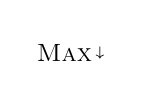
\begin{tikzpicture}[xscale=0.6,yscale=0.4]
\node (max) at (0,0) {{\small \textsc{Max}}};
\node (reg) at (0.75,0.5) {{\fns \textalpha}};
\node (arrow) at (0.75,0) {{\tiny $\downarrow$}};
\node (Rt) at (0.75,-0.5) {{\fns \textbeta}};
\end{tikzpicture}
\end{minipage}
}

\newcommand{\DepAB}{
\begin{minipage}{0.09\textwidth}
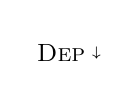
\begin{tikzpicture}[xscale=0.6,yscale=0.4]
\node (max) at (0,0) {{\small \textsc{Dep}}};
\node (reg) at (0.75,0.5) {{\fns \textalpha}};
\node (arrow) at (0.75,0) {{\tiny $\downarrow$}};
\node (Rt) at (0.75,-0.5) {{\fns \textbeta}};
\end{tikzpicture}
\end{minipage}
}

\newcommand{\DepHReg}{
\begin{minipage}{0.055\textwidth}
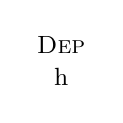
\begin{tikzpicture}[xscale=0.6,yscale=0.4]
\node (dep) at (0,0) {{\small \textsc{Dep}}};
\node (reg) at (0,-1.0) {{\small h}};
\end{tikzpicture}
\end{minipage}
}

\newcommand{\DepLReg}{
\begin{minipage}{0.055\textwidth}
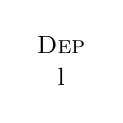
\begin{tikzpicture}[xscale=0.6,yscale=0.4]
\node (dep) at (0,0) {{\small \textsc{Dep}}};
\node (reg) at (0,-1.0) {{\small l}};
\end{tikzpicture}
\end{minipage}
}

\newcommand{\DepReg}{
\begin{minipage}{0.055\textwidth}
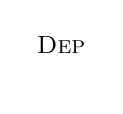
\begin{tikzpicture}[xscale=0.6,yscale=0.4]
\node (dep) at (0,0) {{\small \textsc{Dep}}};
\node (reg) at (0,-1.0) {{\small \textrho}};
\end{tikzpicture}
\end{minipage}
}

\newcommand{\DepTRt}{
\begin{minipage}{0.1\textwidth}
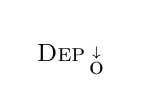
\begin{tikzpicture}[xscale=0.6,yscale=0.4]
\node (dep) at (0,0) {{\small \textsc{Dep}}};
\node (t) at (0.75,0.5) {{\fns \texttau}};
\node (arrow) at (0.75,0) {{\tiny $\downarrow$}};
\node (Rt) at (0.75,-0.5) {{\fns o}};
\end{tikzpicture}
\end{minipage}
}

\newcommand{\MaxRegRt}{
\begin{minipage}{0.1\textwidth}
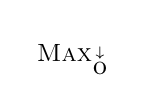
\begin{tikzpicture}[xscale=0.6,yscale=0.4]
\node (max) at (0,0) {{\small \textsc{Max}}};
\node (arrow) at (0.75,0) {{\tiny $\downarrow$}};
\node (Rt) at (0.75,-0.5) {{\fns o}};
\node (reg) at (0.75,0.5) {{\fns \textrho}};
\end{tikzpicture}
\end{minipage}
}

\newcommand{\RegToneByRt}{
\begin{minipage}{0.06\textwidth}
\begin{tikzpicture}[xscale=0.6,yscale=0.5]
\node[rotate=20] (arrow1) at (-0.15,0) {{\fns $\uparrow$}};
\node[rotate=340] (arrow2) at (0.15,0) {{\fns $\uparrow$}};
\node (Rt) at (0,-0.55) {{\small o}};
\node (reg) at (0.4,0.55) {{\small \textrho}};
\node (tone) at (-0.4,0.55) {{\small \texttau}};
\end{tikzpicture}
\end{minipage}
}

\newcommand{\RegToneBySyl}{
\begin{minipage}{0.06\textwidth}
\begin{tikzpicture}[xscale=0.6,yscale=0.5]
\node[rotate=20] (arrow1) at (-0.15,0) {{\fns $\uparrow$}};
\node[rotate=340] (arrow2) at (0.15,0) {{\fns $\uparrow$}};
\node (Rt) at (0,-0.55) {{\small \textsigma}};
\node (reg) at (0.4,0.55) {{\small \textrho}};
\node (tone) at (-0.4,0.55) {{\small \texttau}};
\end{tikzpicture}
\end{minipage}
}

\newcommand{\DepTone}{
\begin{minipage}{0.055\textwidth}
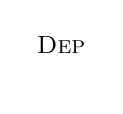
\begin{tikzpicture}[xscale=0.6,yscale=0.4]
\node (dep) at (0,0) {{\small \textsc{Dep}}};
\node (tone) at (0,-1.0) {{\small \texttau}};
\end{tikzpicture}
\end{minipage}
}

\newcommand{\DepTonalRt}{
\begin{minipage}{0.055\textwidth}
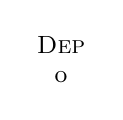
\begin{tikzpicture}[xscale=0.6,yscale=0.4]
\node (dep) at (0,0) {{\small \textsc{Dep}}};
\node (tone) at (0,-1.0) {{\small o}};
\end{tikzpicture}
\end{minipage}
}

\newcommand{\DepL}{
\begin{minipage}{0.055\textwidth}
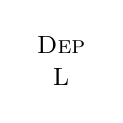
\begin{tikzpicture}[xscale=0.6,yscale=0.4]
\node (dep) at (0,0) {{\small \textsc{Dep}}};
\node (tone) at (0,-1.0) {{\small L}};
\end{tikzpicture}
\end{minipage}
}

\newcommand{\DepH}{
\begin{minipage}{0.055\textwidth}
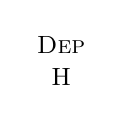
\begin{tikzpicture}[xscale=0.6,yscale=0.4]
\node (dep) at (0,0) {{\small \textsc{Dep}}};
\node (tone) at (0,-1.0) {{\small H}};
\end{tikzpicture}
\end{minipage}
}

\newcommand{\NoMultDiff}{{\small *loh}}
\newcommand{\Alt}{{\small \textsc{Alt}}}
\newcommand{\NoSkip}{{\small \scell{\textsc{No}\\\textsc{Skip}}}}


\newcommand{\RegDomRt}{
\begin{minipage}{0.030\textwidth}
\begin{tikzpicture}[xscale=0.6,yscale=0.5]
\node (arrow) at (0,0) {{\fns $\downarrow$}};
\node (Rt) at (0,-0.55) {{\small o}};
\node (reg) at (0,0.55) {{\small \textrho}};
\end{tikzpicture}
\end{minipage}
}

\newcommand{\DepRegRt}{
\begin{minipage}{0.1\textwidth}
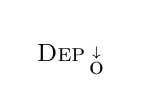
\begin{tikzpicture}[xscale=0.6,yscale=0.4]
\node (dep) at (0,0) {{\small \textsc{Dep}}};
\node (arrow) at (0.75,0) {{\tiny $\downarrow$}};
\node (Rt) at (0.75,-0.5) {{\fns o}};
\node (reg) at (0.75,0.5) {{\fns \textrho}};
\end{tikzpicture}
\end{minipage}
}

% unused

\newcommand{\ToneByRt}{
\begin{minipage}{0.05\textwidth}
\begin{tikzpicture}[xscale=0.6,yscale=0.5]
\node (arrow) at (0,0) {{\fns $\uparrow$}};
\node (Rt) at (0,-0.55) {{\small o}};
\node (tone) at (0,0.55) {{\small \texttau}};
\end{tikzpicture}
\end{minipage}
}

\newcommand{\RegByRt}{
\begin{minipage}{0.05\textwidth}
\begin{tikzpicture}[xscale=0.6,yscale=0.5]
\node (arrow) at (0,0) {{\fns $\uparrow$}};
\node (Rt) at (0,-0.55) {{\small o}};
\node (reg) at (0,0.55) {{\small \textrho}};
\end{tikzpicture}
\end{minipage}
}

\newcommand{\ToneDomRt}{
\begin{minipage}{0.05\textwidth}
\begin{tikzpicture}[xscale=0.6,yscale=0.5]
\node (arrow) at (0,0) {{\fns $\downarrow$}};
\node (Rt) at (0,-0.55) {{\small o}};
\node (tone) at (0,0.55) {{\small \texttau}};
\end{tikzpicture}
\end{minipage}
}

% --- OT tableaus --- %

% Sec. 3.2, first tabl.

\newcommand{\OTHLInput}{
\begin{minipage}{0.17\textwidth}
\begin{tikzpicture}[xscale=\myscalex,yscale=\myscaley]
\node (tone) at (2,0) {(= H)};
\node (syl) at (0,0) {\textsigma};
\node (Rt) at (0,1) {o};
\node (H) at (-0.5,2) {H};
\node (R) at (0.5,3) {h};
\node (Rt2) at (1.5,1.0) {o};
%\node (H2) at (1.0,2) {\epen{L}};
\node (R2) at (2.0,3) {\blue{l}};
\draw [thick] (syl.north) -- (Rt.south) ;
\draw [thick] (Rt.north) -- (H.south) ;
\draw [thick] (Rt.north) -- (R.south) ;
\draw [thick] (syl.north) -- (Rt2.south) ;
%\draw [dashed] (Rt2.north) -- (H2.south) ;
%\draw [dashed] (Rt2.north) -- (R2.south) ;
\end{tikzpicture}
\end{minipage}
}

\newcommand{\OTHLWinner}{
\begin{minipage}{0.17\textwidth}
\begin{tikzpicture}[xscale=\myscalex,yscale=\myscaley]
\node (tone) at (2,0) {(= HL)};
\node (syl) at (0,0) {\textsigma};
\node (Rt) at (0,1) {o};
\node (H) at (-0.5,2) {H};
\node (R) at (0.5,3) {h};
\node (Rt2) at (1.5,1.0) {o};
\node (H2) at (1.0,2) {\epen{L}};
\node (R2) at (2.0,3) {\blue{l}};
\draw [thick] (syl.north) -- (Rt.south) ;
\draw [thick] (Rt.north) -- (H.south) ;
\draw [thick] (Rt.north) -- (R.south) ;
\draw [thick] (syl.north) -- (Rt2.south) ;
\draw [dashed] (Rt2.north) -- (H2.south) ;
\draw [dashed] (Rt2.north) -- (R2.south) ;
\end{tikzpicture}
\end{minipage}
}

\newcommand{\OTHLSpreadingHOnly}{
\begin{minipage}{0.17\textwidth}
\begin{tikzpicture}[xscale=\myscalex,yscale=\myscaley]
\node (tone) at (2,0) {(= HM)};
\node (syl) at (0,0) {\textsigma};
\node (Rt) at (0,1) {o};
\node (H) at (-0.5,2) {H};
\node (R) at (0.5,3) {h};
\node (Rt2) at (1.5,1.0) {o};
%\node (H2) at (1.0,2) {\epen{L}};
\node (R2) at (2.0,3) {\blue{l}};
\draw [thick] (syl.north) -- (Rt.south) ;
\draw [thick] (Rt.north) -- (H.south) ;
\draw [thick] (Rt.north) -- (R.south) ;
\draw [thick] (syl.north) -- (Rt2.south) ;
\draw [dashed] (Rt2.north) -- (R2.south) ;
\draw [dashed] (Rt2.north) -- (H.south) ;
\end{tikzpicture}
\end{minipage}
}

\newcommand{\OTHLInsertH}{
\begin{minipage}{0.17\textwidth}
\begin{tikzpicture}[xscale=\myscalex,yscale=\myscaley]
\node (tone) at (2,0) {(= HM)};
\node (syl) at (0,0) {\textsigma};
\node (Rt) at (0,1) {o};
\node (H) at (-0.5,2) {H};
\node (R) at (0.5,3) {h};
\node (Rt2) at (1.5,1.0) {o};
\node (H2) at (1.0,2) {\epen{H}};
\node (R2) at (2.0,3) {\blue{l}};
\draw [thick] (syl.north) -- (Rt.south) ;
\draw [thick] (Rt.north) -- (H.south) ;
\draw [thick] (Rt.north) -- (R.south) ;
\draw [thick] (syl.north) -- (Rt2.south) ;
\draw [dashed] (Rt2.north) -- (H2.south) ;
\draw [dashed] (Rt2.north) -- (R2.south) ;
\end{tikzpicture}
\end{minipage}
}

\newcommand{\OTHLOverwriting}{
\begin{minipage}{0.17\textwidth}
\begin{tikzpicture}[xscale=\myscalex,yscale=\myscaley]
\node (syl) at (0,0) {\textsigma};
\node (Rt) at (0,1) {o};
\node (H) at (-0.5,2) {H};
\node (R) at (0.5,3) {h};
\node (Rt2) at (1.5,1.0) {o};
%\node (H2) at (1.0,2) {\epen{L}};
\node (R2) at (2.0,3) {\blue{l}};
\draw [thick] (syl.north) -- (Rt.south) ;
\draw [thick] (Rt.north) -- (H.south) ;
\draw [thick] (Rt.north) -- (R.south) ;
\draw [thick] (syl.north) -- (Rt2.south) ;
%\draw [dashed] (Rt2.north) -- (H2.south) ;
\draw [dashed] (Rt.north) -- (R2.south) ;
\node (del) at (0.3,1.9) {\textbf{=}};
\end{tikzpicture}
\end{minipage}
}

\newcommand{\OTHLSpreading}{
\begin{minipage}{0.17\textwidth}
\begin{tikzpicture}[xscale=\myscalex,yscale=\myscaley]
\node (syl) at (0,0) {\textsigma};
\node (Rt) at (0,1) {o};
\node (H) at (-0.5,2) {H};
\node (R) at (0.5,3) {h};
\node (Rt2) at (1.5,1.0) {o};
%\node (H2) at (1.0,2) {\epen{L}};
\node (R2) at (2.0,3) {\blue{l}};
\draw [thick] (syl.north) -- (Rt.south) ;
\draw [thick] (Rt.north) -- (H.south) ;
\draw [thick] (Rt.north) -- (R.south) ;
\draw [thick] (syl.north) -- (Rt2.south) ;
%\draw [dashed] (Rt2.north) -- (H2.south) ;
\draw [dashed] (Rt2.north) -- (H.south) ;
\draw [dashed] (Rt2.north) -- (R.south) ;
\end{tikzpicture}
\end{minipage}
}

% Sec. 4.2, second tabl.: phrase-medial position

\newcommand{\OTHnoLInput}{
\begin{minipage}{0.17\textwidth}
\begin{tikzpicture}[xscale=\myscalex,yscale=\myscaley]
\node (tone) at (2,0) {(= H)};
\node (syl) at (0,0) {\textsigma};
\node (Rt) at (0,1) {o};
\node (H) at (-0.5,2) {H};
\node (R) at (0.5,3) {h};
\node (Rt2) at (1.5,1.0) {o};
%\node (H2) at (1.0,2) {\epen{L}};
%\node (R2) at (2.0,3) {\blue{l}};
\draw [thick] (syl.north) -- (Rt.south) ;
\draw [thick] (Rt.north) -- (H.south) ;
\draw [thick] (Rt.north) -- (R.south) ;
\draw [thick] (syl.north) -- (Rt2.south) ;
\end{tikzpicture}
\end{minipage}
}

\newcommand{\OTHnoLEpenth}{
\begin{minipage}{0.17\textwidth}
\begin{tikzpicture}[xscale=\myscalex,yscale=\myscaley]
\node (tone) at (2,0) {(= HM)};
\node (syl) at (0,0) {\textsigma};
\node (Rt) at (0,1) {o};
\node (H) at (-0.5,2) {H};
\node (R) at (0.5,3) {h};
\node (Rt2) at (1.5,1.0) {o};
\node (H2) at (1.0,2) {\epen{L}};
\node (R2) at (2.0,3) {\epen{h}};
\draw [thick] (syl.north) -- (Rt.south) ;
\draw [thick] (Rt.north) -- (H.south) ;
\draw [thick] (Rt.north) -- (R.south) ;
\draw [thick] (syl.north) -- (Rt2.south) ;
\draw [dashed] (Rt2.north) -- (H2.south) ;
\draw [dashed] (Rt2.north) -- (R2.south) ;
\end{tikzpicture}
\end{minipage}
}

\newcommand{\OTHnoLSpreading}{
\begin{minipage}{0.17\textwidth}
\begin{tikzpicture}[xscale=\myscalex,yscale=\myscaley]
\node (tone) at (2,0) {(= HH)};
\node (syl) at (0,0) {\textsigma};
\node (Rt) at (0,1) {o};
\node (H) at (-0.5,2) {H};
\node (R) at (0.5,3) {h};
\node (Rt2) at (1.5,1.0) {o};
%\node (H2) at (1.0,2) {\epen{L}};
%\node (R2) at (2.0,3) {\blue{l}};
\draw [thick] (syl.north) -- (Rt.south) ;
\draw [thick] (Rt.north) -- (H.south) ;
\draw [thick] (Rt.north) -- (R.south) ;
\draw [thick] (syl.north) -- (Rt2.south) ;
\draw [dashed] (Rt2.north) -- (H.south) ;
\draw [dashed] (Rt2.north) -- (R.south) ;
\end{tikzpicture}
\end{minipage}
}

% Sec. 4.2, third tabl., LM is unaffected by L\%

\newcommand{\OTLMInput}{
\begin{minipage}{0.2\textwidth}
\begin{tikzpicture}[xscale=\myscalex,yscale=\myscaley]
\node (tone) at (2,0) {(= LM)};
\node (syl) at (0,0) {\textsigma};
\node (Rt) at (0,1) {o};
\node (H) at (-0.5,2) {L};
\node (R) at (0.5,3) {l};
\node (Rt2) at (1.5,1.0) {o};
\node (H2) at (1.0,2) {L};
\node (R2) at (2.0,3) {h};
\node (R3) at (3.0,3) {\blue{l}};
\draw [thick] (syl.north) -- (Rt.south) ;
\draw [thick] (Rt.north) -- (H.south) ;
\draw [thick] (Rt.north) -- (R.south) ;
\draw [thick] (syl.north) -- (Rt2.south) ;
\draw [thick] (Rt2.north) -- (H2.south) ;
\draw [thick] (Rt2.north) -- (R2.south) ;
\end{tikzpicture}
\end{minipage}
}

\newcommand{\OTLMReplace}{
\begin{minipage}{0.2\textwidth}
\begin{tikzpicture}[xscale=\myscalex,yscale=\myscaley]
\node (tone) at (2,0) {(= LL)};
\node (syl) at (0,0) {\textsigma};
\node (Rt) at (0,1) {o};
\node (H) at (-0.5,2) {L};
\node (R) at (0.5,3) {l};
\node (Rt2) at (1.5,1.0) {o};
\node (H2) at (1.0,2) {L};
\node (R2) at (2.0,3) {h};
\node (R3) at (3.0,3) {\blue{l}};
\draw [thick] (syl.north) -- (Rt.south) ;
\draw [thick] (Rt.north) -- (H.south) ;
\draw [thick] (Rt.north) -- (R.south) ;
\draw [thick] (syl.north) -- (Rt2.south) ;
\draw [thick] (Rt2.north) -- (H2.south) ;
\draw [thick] (Rt2.north) -- (R2.south) ;
\draw [dashed] (Rt2.north) -- (R3.south) ;
\node (del) at (1.8,2.1) {\textbf{=}};
\end{tikzpicture}
\end{minipage}
}

\newcommand{\OTLMTwoReg}{
\begin{minipage}{0.2\textwidth}
\begin{tikzpicture}[xscale=\myscalex,yscale=\myscaley]
\node (tone) at (2,0) {(= LML)};
\node (syl) at (0,0) {\textsigma};
\node (Rt) at (0,1) {o};
\node (H) at (-0.5,2) {L};
\node (R) at (0.5,3) {l};
\node (Rt2) at (1.5,1.0) {o};
\node (H2) at (1.0,2) {L};
\node (R2) at (2.0,3) {h};
\node (R3) at (3.0,3) {\blue{l}};
\draw [thick] (syl.north) -- (Rt.south) ;
\draw [thick] (Rt.north) -- (H.south) ;
\draw [thick] (Rt.north) -- (R.south) ;
\draw [thick] (syl.north) -- (Rt2.south) ;
\draw [thick] (Rt2.north) -- (H2.south) ;
\draw [thick] (Rt2.north) -- (R2.south) ;
\draw [dashed] (Rt2.north) -- (R3.south) ;
\end{tikzpicture}
\end{minipage}
}

% Sec. 4.2, fourth tabl., L is affected by L\% but M is not

\newcommand{\OTLInput}{
\begin{minipage}{0.17\textwidth}
\begin{tikzpicture}[xscale=\myscalex,yscale=\myscaley]
\node (tone) at (2,0) {(= L)};
\node (syl) at (0,0) {\textsigma};
\node (Rt) at (0,1) {o};
\node (H) at (-0.5,2) {L};
\node (R) at (0.5,3) {l};
\node (R2) at (2,3) {\blue{l}};
\draw [thick] (syl.north) -- (Rt.south) ;
\draw [thick] (Rt.north) -- (H.south) ;
\draw [thick] (Rt.north) -- (R.south) ;
\end{tikzpicture}
\end{minipage}
}

\newcommand{\OTLLowered}{
\begin{minipage}{0.17\textwidth}
\begin{tikzpicture}[xscale=\myscalex,yscale=\myscaley]
\node (tone) at (2,0) {(= LL)};
\node (syl) at (0,0) {\textsigma};
\node (Rt) at (0,1) {o};
\node (H) at (-0.5,2) {L};
\node (R) at (0.5,3) {l};
\node (R2) at (2,3) {\blue{l}};
\draw [thick] (syl.north) -- (Rt.south) ;
\draw [thick] (Rt.north) -- (H.south) ;
\draw [thick] (Rt.north) -- (R.south) ;
\draw [dashed] (Rt.north) -- (R2.south) ;
\end{tikzpicture}
\end{minipage}
}

\newcommand{\OTMInput}{
\begin{minipage}{0.17\textwidth}
\begin{tikzpicture}[xscale=\myscalex,yscale=\myscaley]
\node (tone) at (2,0) {(= M)};
\node (syl) at (0,0) {\textsigma};
\node (Rt) at (0,1) {o};
\node (H) at (-0.5,2) {L};
\node (R) at (0.5,3) {h};
\node (R2) at (2,3) {\blue{l}};
\draw [thick] (syl.north) -- (Rt.south) ;
\draw [thick] (Rt.north) -- (H.south) ;
\draw [thick] (Rt.north) -- (R.south) ;
\end{tikzpicture}
\end{minipage}
}

\newcommand{\OTMLowered}{
\begin{minipage}{0.17\textwidth}
\begin{tikzpicture}[xscale=\myscalex,yscale=\myscaley]
\node (tone) at (2,0) {(= ML)};
\node (syl) at (0,0) {\textsigma};
\node (Rt) at (0,1) {o};
\node (H) at (-0.5,2) {L};
\node (R) at (0.5,3) {h};
\node (R2) at (2,3) {\blue{l}};
\draw [thick] (syl.north) -- (Rt.south) ;
\draw [thick] (Rt.north) -- (H.south) ;
\draw [thick] (Rt.north) -- (R.south) ;
\draw [dashed] (Rt.north) -- (R2.south) ;
\end{tikzpicture}
\end{minipage}
}

% Sec. 4.2, fifth tableau, polar questions with level tones

\newcommand{\OTLPolIn}{
\begin{minipage}{0.20\textwidth}
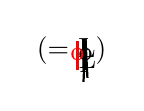
\begin{tikzpicture}[xscale=\myscalex-0.05,yscale=\myscaley-0.05]
\node (tone) at (3.5,0) {(= L)};
\node (syl) at (0,0) {\textsigma};
\node (syl2) at (2,0) {\red{\textsigma}};
\node (Rt) at (0,1) {o};
\node (H) at (-0.5,2) {L};
\node (R) at (0.5,3) {l};
\node (Rt2) at (2,1) {\red{o}};
\draw [thick] (syl.north) -- (Rt.south) ;
\draw [thick,red] (syl2.north) -- (Rt2.south) ;
\draw [thick] (Rt.north) -- (H.south) ;
\draw [thick] (Rt.north) -- (R.south) ;
\end{tikzpicture}
\end{minipage}
}

\newcommand{\OTLPolDef}{
\begin{minipage}{0.20\textwidth}
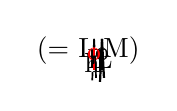
\begin{tikzpicture}[xscale=\myscalex-0.05,yscale=\myscaley-0.05]
\node (tone) at (3.5,0) {(= L.M)};
\node (syl) at (0,0) {\textsigma};
\node (syl2) at (2,0) {\red{\textsigma}};
\node (Rt) at (0,1) {o};
\node (H) at (-0.5,2) {L};
\node (R) at (0.5,3) {l};
\node (H2) at (1.5,2) {\epen{L}};
\node (R2) at (2.5,3) {\epen{h}};
\node (Rt2) at (2,1) {\red{o}};
\draw [thick] (syl.north) -- (Rt.south) ;
\draw [thick,red] (syl2.north) -- (Rt2.south) ;
\draw [thick] (Rt.north) -- (H.south) ;
\draw [thick] (Rt.north) -- (R.south) ;
\draw [semithick,dashed] (Rt2.north) -- (H2.south) ;
\draw [semithick,dashed] (Rt2.north) -- (R2.south) ;
\end{tikzpicture}
\end{minipage}
}

\newcommand{\OTLPolAlt}{
\begin{minipage}{0.20\textwidth}
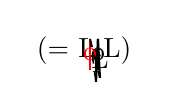
\begin{tikzpicture}[xscale=\myscalex-0.05,yscale=\myscaley-0.05]
\node (tone) at (3.5,0) {(= L.L)};
\node (syl) at (0,0) {\textsigma};
\node (syl2) at (2,0) {\red{\textsigma}};
\node (Rt) at (0,1) {o};
\node (H) at (-0.5,2) {L};
\node (R) at (0.5,3) {l};
\node (Rt2) at (2,1) {\red{o}};
\draw [thick] (syl.north) -- (Rt.south) ;
\draw [thick,red] (syl2.north) -- (Rt2.south) ;
\draw [thick] (Rt.north) -- (H.south) ;
\draw [thick] (Rt.north) -- (R.south) ;
\draw [semithick,dashed] (Rt2.north) -- (H.south) ;
\draw [semithick,dashed] (Rt2.north) -- (R.south) ;
\end{tikzpicture}
\end{minipage}
}

% Sec. 4.2, sixth tableau, polar questions with contour tones

\newcommand{\OTLLPolIn}{
\begin{minipage}{0.23\textwidth}
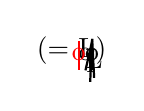
\begin{tikzpicture}[xscale=\myscalex-0.05,yscale=\myscaley-0.05]
\node (tone) at (5.2,0) {(= L)};
\node (syl) at (0,0) {\textsigma};
\node (syl3) at (3.4,0) {\red{\textsigma}};
\node (Rt) at (0,1) {o};
\node (Rt2) at (1.7,1) {o};
\node (Rt3) at (3.4,1) {\red{o}};
\node (H) at (-0.5,2) {L};
\node (R) at (0.5,3) {l};
\draw [thick] (syl.north) -- (Rt.south) ;
\draw [thick] (syl.north) -- (Rt2.south) ;
\draw [thick,red] (syl3.north) -- (Rt3.south) ;
\draw [thick] (Rt.north) -- (H.south) ;
\draw [thick] (Rt.north) -- (R.south) ;
\end{tikzpicture}
\end{minipage}
}

\newcommand{\OTLLPolDef}{
\begin{minipage}{0.23\textwidth}
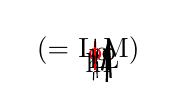
\begin{tikzpicture}[xscale=\myscalex-0.05,yscale=\myscaley-0.05]
\node (tone) at (5.2,0) {(= L.M)};
\node (syl) at (0,0) {\textsigma};
\node (syl3) at (3.4,0) {\red{\textsigma}};
\node (Rt) at (0,1) {o};
\node (Rt2) at (1.7,1) {o};
\node (Rt3) at (3.4,1) {\red{o}};
\node (H) at (-0.5,2) {L};
\node (R) at (0.5,3) {l};
\node (H3) at (2.9,2) {\epen{L}};
\node (R3) at (3.9,3) {\epen{h}};
\draw [thick] (syl.north) -- (Rt.south) ;
\draw [thick] (syl.north) -- (Rt2.south) ;
\draw [thick,red] (syl3.north) -- (Rt3.south) ;
\draw [thick] (Rt.north) -- (H.south) ;
\draw [thick] (Rt.north) -- (R.south) ;
\draw [dashed] (Rt3.north) -- (H3.south) ;
\draw [dashed] (Rt3.north) -- (R3.south) ;
\end{tikzpicture}
\end{minipage}
}

\newcommand{\OTLLPolSkip}{
\begin{minipage}{0.23\textwidth}
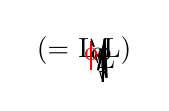
\begin{tikzpicture}[xscale=\myscalex-0.05,yscale=\myscaley-0.05]
\node (tone) at (5.2,0) {(= L.L)};
\node (syl) at (0,0) {\textsigma};
\node (syl3) at (3.4,0) {\red{\textsigma}};
\node (Rt) at (0,1) {o};
\node (Rt2) at (1.7,1) {o};
\node (Rt3) at (3.4,1) {\red{o}};
\node (H) at (-0.5,2) {L};
\node (R) at (0.5,3) {l};
\draw [thick] (syl.north) -- (Rt.south) ;
\draw [thick] (syl.north) -- (Rt2.south) ;
\draw [thick,red] (syl3.north) -- (Rt3.south) ;
\draw [thick] (Rt.north) -- (H.south) ;
\draw [thick] (Rt.north) -- (R.south) ;
\draw [dashed] (Rt3.north) -- (H.south) ;
\draw [dashed] (Rt3.north) -- (R.south) ;
\end{tikzpicture}
\end{minipage}
}  
  
\newcommand{\ilit}[1]{#1\il{#1}}    
\newcommand{\isit}[1]{#1\is{#1}}  

\makeatletter
\let\thetitle\@title
\let\theauthor\@author 
\makeatother

\newcommand{\togglepaper}[1][0]{ 
  \bibliography{../localbibliography}
  %% hyphenation points for line breaks
%% Normally, automatic hyphenation in LaTeX is very good
%% If a word is mis-hyphenated, add it to this file
%%
%% add information to TeX file before \begin{document} with:
%% %% hyphenation points for line breaks
%% Normally, automatic hyphenation in LaTeX is very good
%% If a word is mis-hyphenated, add it to this file
%%
%% add information to TeX file before \begin{document} with:
%% \include{localhyphenation}
\hyphenation{
affri-ca-te
affri-ca-tes
com-ple-ments
par-a-digm
Sha-ron
Kings-ton
phe-nom-e-non
Daul-ton
Abu-ba-ka-ri
Ngo-nya-ni
Clem-ents 
King-ston
Tru-cken-brodt
Tab-leau
cophono-logies
mark-edness
Ti-gri-nya
a-mong
Car-stens
Lu-bu-ku-su
}
\hyphenation{
affri-ca-te
affri-ca-tes
com-ple-ments
par-a-digm
Sha-ron
Kings-ton
phe-nom-e-non
Daul-ton
Abu-ba-ka-ri
Ngo-nya-ni
Clem-ents 
King-ston
Tru-cken-brodt
Tab-leau
cophono-logies
mark-edness
Ti-gri-nya
a-mong
Car-stens
Lu-bu-ku-su
}
  \papernote{\scriptsize\normalfont
    \theauthor.
    \thetitle. 
    To appear in: 
    Emily Clem,   Peter Jenks \& Hannah Sande.
    Theory and description in African Linguistics: Selected papers from the 47th Annual Conference on African Linguistics.
    Berlin: Language Science Press. [preliminary page numbering]
  }
  \pagenumbering{roman}
  \setcounter{chapter}{#1}
  \addtocounter{chapter}{-1}
}

\newcommand{\upstep}{\textupstep}


% \newcounter{tableauxcounter}

\renewcommand{\textltailn}{ɲ}
\renewcommand{\textbardotlessj}{ɟ}

\newcommand{\emphkh}[1]{\textit{#1}} %originally \textbf, banned by the guidelines



\definecolor{lsDOIGray}{cmyk}{0,0,0,0.45}


\newcommand{\xuparrow}[1]{%
  {\left\uparrow\vbox to #1{}\right.\kern-\nulldelimiterspace}
}
\renewcommand \textupstep[1]{\char"A71B#1}
\renewcommand \textdownstep[1]{\char"A71C#1}
 
 \newcommand{\ꜛ}{\textsf{ꜛ}}
 
\def\biberror{\undefined}


\newcommand{\OTbox}[1]{\resizebox{.88\textwidth}{!}{#1}}
 

%\renewcommand{\thefootnote}{\arabic{footnote}} %numbers footnotes %

\author{Betsy Pillion\affiliation{University of Chicago}\and Lenore A. Grenoble\affiliation{University of Chicago}\and Emmanuel Ngu{\'e} Um\affiliation{University of Yaound{\'e}}\lastand Sarah Kopper\affiliation{Michigan State University}}
\title{Verbal gestures in Cameroon} 

\abstract{This paper details the nature of a set of extra-grammatical units that we call \textit{verbal gestures}, found in several communities in the Central, Littoral, and Southern regions of Cameroon. We lay out the verbal gestures found in these communities, explain their usage and distribution within the context of the community and the language of the user, and situate the system of verbal gestures found in Cameroon in the larger linguistic context of Cameroonian multilingualism.  Furthermore, we make preliminary proposals for a system of sounds that exists outside of that of the primary phonemic system, which interacts with the system of verbal gestures. }

\begin{document}
\maketitle

\section{Introduction}

We use the term \textit{verbal gestures} to refer to a set of linguistic elements that  are extra-grammatical, in the sense that they are not used in a morphosyntactic frame, and thus are not lexical words per se, but may serve the same functional purpose. Verbal gestures  often include sounds or segments that stand outside a language's \isi{phonemic inventory}; in many of the documented instances of verbal gestures that we illustrate here, they consist only of non-phonemic segments. Nonetheless, verbal gestures are a core part of the communicative system of the language.  Verbal gestures are readily recognized by speakers as having semantic and pragmatic meaning, but are not words. Examples in \ili{English} include the use of the glottal stop in some pronunciations of \textit{uh-oh} or in the dental \isi{click} in \textit{tsk-tsk}. These sounds, despite not being used in recombinable units within the phonemic system, are consistent in their articulatory execution and acoustic result. We propose that these systematic articulations are governed by a secondary sound system. The level of interaction that this system seems to have with the \isi{primary phonemic system}, and the extent to which these sounds can differ in their articulation, are still open questions. We present a preliminary analysis in \sectref{sec:pillion:secondary}. The present contribution is a part of a larger project investigating the category of verbal gestures cross-linguistically; here we present one small subset resulting from a pilot study conducted by the authors in Cameroon in 2015.

This work builds on previous research on verbal gestures in Senegal \citet{grenobleetal2015}, focusing instead on verbal gestures in Cameroon, and expands the theoretical groundwork of the earlier work. Verbal gestures have much in common with what \citep{wals-142} has identified as \textit{paralinguistic clicks}, but the category of verbal gestures is larger and includes sounds that are not clicks, and includes items that are not paralinguistic but linguistic.\footnote{The term \textit{paralinguistic} has been used to refer to a host of categories over the years. While Gil’s use of \textit{paralinguistic} selects these clicks as being objects in some way alongside language but not within it, many researchers use \textit{paralinguistic} to refer to aspects of speech that are not strictly contrastive or linguistic but indicate other aspects of a person’s voice such as confidence \citep{Scherer197331}, or suprasegmental attributes of the speech signal that signal emotion \citep{Fujisaki1993}. It is for this reason that we avoid the term in categorizing verbal gestures.  See also \citet[112]{ameka1992} who discusses the characterization of interjections as paralinguistic and thus peripheral.} Gil notes that ``paralinguistic clicks resemble other linguistic signs in that they are arbitrary and conventionalized." Since they are vocal, it is unclear what distinguishes them from other linguistic items, such as interjections, except that they contain non-phonemic clicks. It has long been recognized that certain categories -- exclamations, interjections, animal calls, baby talk, foreign words -- often contain sounds not found elsewhere in the sound system, as noted by \citep[71]{harris1951}; see also \citep{friespike}.

The phenomena under investigation here are not discourse markers, defined as
 ``sequentially dependent elements which bracket units of talk'' \citep[31]{schiffrin1987}  or as signaling  a relationship between the upcoming message and prior discourse \citep{fraser1990, fraser1996, fraser1999} and have a ``core meaning that is procedural, not conceptual'' \citep[950]{fraser1999}. With reference to manual gestures, these have been called \textit{discourse unit markers}, ``labels for segments or units within a discourse, thereby indicating the part these units play within the discourse structure'' \citep[248]{kendon1995}. We add to a growing body of research on phenomena that have been historically considered to be on the margins of language, but have increasingly been analyzed as integral to the overall communicative situation. Examples include phenomena with unusual sounds, such whistle speech \citep{meyer2015, sicoli2016}, hesitation markers \citep{dingemanse2013plos, schegloff1982}, ideophones \citep{childs1994}, and theticals \citep{kaltenbocketal2011}, which are prosodically distinct and syntactically independent.
 

Verbal gestures are perhaps best viewed as a subset of the larger category of interjections, a class generally defined as including both word types and an utterance type \citep[102]{ameka1992}. The word types constitute a special subset because of their particular phonetic and morphosyntactic properties: they are often phonologically distinctive, and may contain sounds not in the \isi{phonemic inventory},  a characteristic of the category of interjections as a whole  \citep{schachter1985}. This category has been referred to as \textit{non-words}. These are primary interjections and ``do not normally enter into construction with other word classes''  \citep[105]{ameka1992}; they are phonologically and morphologically anomalous. The class of verbal gestures as we define it is sufficiently broad to include  phenomena that  are similar to \textit{quotable gestures} or \textit{emblems}  which  include\textit{ lexical gestures} that can be translated into lexical words \citep{brookes2004, poggi1983, poggizomparelli1987}. In these respects verbal gestures are very much like quotable gestures, but they are vocal, not manual or facial. They differ from lexical words in each of the languages examined in our fieldwork in that they not only do not take morphology, but also cannot be embedded. (For more detailed discussion, see \citealt{grenobleetal2015}.)  

Verbal gestures do not enter into a morphosyntactic frame: they do not combine with the grammar, or inflectional or derivational morphology. They have conventional content and form: they are  readily understood and used by multiple speakers across the \isi{speech community}. They  can constitute an utterance. Like other utterances, they may overlap with another speaker's utterance, or they may stand alone, for example as a second-pair part of an adjacency pair.
%(\citet[102]{ameka1992}).
Verbal gestures are readily borrowable cross-linguistically, precisely because they do not enter into a morphosyntactic frame and are attractive because they make use of sounds that are highly salient to outside speakers. 

The verbal gestures we have documented in Cameroon are very similar across different languages, with some differences in production.  For example, the gesture for negative affect is similar in all tested regions of Cameroon and across speakers of different mother tongues, but varies in terms of the duration of the gesture and head \isi{movement}.  
%\citet{schachter1985}

%Previous research from Lenore and colleagues about what verbal gestures are.
In contrast to verbal gestures in Cameroon,  \ili{Wolof} speakers in Senegal use a \textit{highly} conventionalized system of verbal gestures, whose meanings and articulations vary minimally. Included in this system are verbal gestures that have the same function as the words `no' and `yes' \citep{grenobleetal2015}.  The systems of verbal gestures we have observed in certain areas of Cameroon differ from those of \ili{Senegalese Wolof} in their level of conventionalization, and there are major differences in the delineation of these systems with respect to how the phonemic system and the verbal gestural system interact. 

Conventionalization involves diachronic patterns of change and is ``typically in a state of flux'' \citep[27]{ferguson1994}; note that \citet[106]{ameka1992} defines interjections as ``relatively conventionalized vocal gestures,'' suggesting a continuum. Conventionalization is thus an ongoing process,  and we take level of conventionalization as a rough reflection of both the consistency of the gesture's pragmatic use within the linguistic system and the consistency of articulatory production. Verbal gestures that are unconventionalized, or lowest on the scale of conventionalization, include nonce gestures, that are uttered once and may have clear contextual meaning, but are not   reproduced by other speakers. More conventionalized verbal gestures have propagated and are found in the wider \isi{speech community}, but are very contextually dependent  for  pragmatic interpretation, or do not have a consistent meaning across the \isi{speech community} but are more widely used than one-off verbal gestures. Finally, conventionalized verbal gestures are consistent in  pragmatic interpretation across the \isi{speech community}, and although each \isi{verbal gesture} may serve multiple functions, its interpretation within a given context is predictable and transparent to interlocutors.
  
Our work is similar in spirit to \citet{eastmanomar1985}, which identifies a special category of co-speech gestures in \ili{Swahili}, placing it on a continuum of verbal--non-verbal communication.  Their work focuses on manual co-speech (or, in their terms, verbally-dependent) gestures, while we are concerned with gestures that are vocalizations, although they may be accompanied by some physical body \isi{movement} (manual gesture, facial expression, head \isi{movement}, or body \isi{movement}). The inventory of \ili{Swahili} interjections includes at least one  ``nonlinguistic vocalization,'' \textit{hng'\textipa{P}ng'}, described as a bisyllabic item, consisting of  ``breathy syllabic \isi{velar nasal} followed by a glottal catch and another syllabic \isi{velar nasal}'' (\citealt{eastman1992}: 281; \citealt{eastmanomar1985}: 328); this sound is accompanied by a distinctive manual gesture to indicate a bad smell. Eastman's study of \ili{Swahili} interjections provides a list of 28 items, many of which are clearly words by any definition, such as \textit{harambee!} `let's all pull/work together'. The gesture \textit{hng'\textipa{P}ng'} is distinct in this regard: it is not a word form, but a \isi{verbal gesture} as defined here.

%(\citealt{eastman1992}: 281; \citealt{eastmanomar1985}: 328)
It should also be noted that in our discussion of verbal gestural systems, we are only able to offer a snapshot of what is  assuredly a varied and multifaceted group of verbal gestures, as of yet undocumented. The scales given here are intended only to serve as a reference for the possibilities of groupings that may exist throughout languages,\footnote{While it is theoretically possible that a language does not use any primary phonemes in its verbal gestures,  that seems highly unlikely and we know of no such system.} and reflect only the gestures that we have documented and are well attested in our field recordings. 

\ili{Wolof} verbal gestures are highly conventionalized. The sounds that these gestures are composed of vary minimally, with the exception of the \textit{waaw} `yes' gesture, which can be produced as an alveolar, palatal, or lateral \isi{click}, apparently in \isi{free variation}. Many \ili{Wolof} verbal gestures use a secondary set of sounds, while also making some use of the \isi{primary phonemic system}. This is illustrated in \figref{fig:pillion:senegal}.  
	%Talk about those funny scales
	
\begin{figure}  
%\ex \ili{Senegalese Wolof} \label{senegal} \\
\includegraphics[scale=0.13]{figures/senegalsystem.jpg}\\
\caption{Senegalese Wolof}
\label{fig:pillion:senegal}
\end{figure}
%\vspace{-3em}
\noindent
\figref{fig:pillion:senegal} illustrates the relationship of verbal gestures to words along the two continua of the sound system and conventionalization.  The lines in the figure indicate that these items exist over a wider range of levels of conventionalization and phonemic statuses and not the total inventory. That is, the figure should not be interpreted as claiming that the inventory of verbal gestures is larger than that of lexical words, but simply that there is more variety with respect to these parameters within that category. 

\ili{Wolof} also has a rich system of ideophones, which function like conventional words in that they take morphology and syntax, and use only phonemic sounds.  They do not use  clicks, unlike many \ili{Wolof} verbal gestures. In contrast, in the Cameroonian languages studied here, verbal gestures are less conventionalized than words, as illustrated in \figref{fig:pillion:cam}.


\begin{figure} 
%\ex Cameroonian Verbal Gestures \label{cam} \\
\includegraphics[scale=0.15]{figures/cameroonsystem.jpg}\\
\caption{Cameroonian verbal gestures}
\label{fig:pillion:cam}
\end{figure}

Cameroonian verbal gestures are varied across languages and areas, but across these systems, we note that even within languages and communities there is less conventionalization of the meaning of these gestures in Cameroon. They are not as readily recognized as they are in \ili{Wolof} communities by speakers, and they have a wider range of possible interpretations (although there are some verbal gestures that are extremely similar between Senegal and Cameroon, see \sectref{subsec:pillion:AttentionGetting} and \sectref{subsec:pillion:NegativeAffect}). The extent to which this lesser level of conventionalization might be related to the multilingualism of the communities in question is not known. This level of conventionalization also may vary from community to community, but in our glimpse of these systems, we note that these gestures do not seem to take the place of words such as in the system in Senegal. 

Despite the differences in the levels of conventionalization between \ili{Wolof} and Cameroonian verbal gestures, there are striking similarities between them in meaning and articulation, as illustrated in \sectref{sec:pillion:vg}. 


\section{Methodology}

Our analysis is based on fieldwork conducted in Cameroon in 2015 in three urban centers (Buea, Ed\'{e}a, Yaound\'{e}), and on the palm oil plantation Apouh A Ngok (Littoral region, to the south of Ed\'{e}a), and casual observations in Douala.  Several methods were employed to elicit and understand verbal gestures: focused elicitation sessions, participant observation, and casual observations while walking around town, including some recordings in the marketplace. Elicitations were conducted in Basa\'{a}, \ili{English}, and \ili{French}. Since Ngu\'{e} Um is a native speaker of Basa\'{a}, we were able to document approximately 90 minutes of spontaneous, unplanned conversation in Basa\'{a}, in two different settings, once with the authors, and once without any of the authors present. In addition, we conducted language surveys in Apouh A Ngok to judge levels of multilingualism. Similar to \citet[191]{brookes2004}, we identify conventional gestures by one of the following criteria: (1) the gesture was attested on more than one occasion in spontaneous speech, signaling a similar meaning; (2) the gesture was observed in spontaneous speech and its usage and meaning were confirmed by a native speaker other than the interlocutor who originally produced it; and (3) it was elicited from multiple native speakers of the same language. Gestures which were claimed to be used by only one native speaker and not otherwise attested in spontaneous speech are given in \tabref{tab:pillion:less}, \sectref{sec:pillion:less}.

Previous work on \ili{Wolof} verbal gestures in Senegal showed them to be very easy to elicit: \ili{Wolof} speakers quickly recognize the phenomenon and readily produce gestures from a description of the semantic/pragmatic content once they understand the question. For example, if asked how to say `yes' (or \textit{oui}) using a sound on the lips, they produce one of three possible \isi{click} variants for this gesture, and easily offer additional verbal gestures. This was not the case in Cameroon, where speakers responded with \textit{mhmm} or \textit{mmm}, starting out with a mid-level pitch and rising at the end, but critically not a \isi{click} (reflecting in part the absence of \textsc {yes/no} gestures in the Cameroonian languages under investigation).  The exception is the production of the negative affect \isi{click}, which is readily elicitable and is referred to in Basa\'{a} as \textit{\tS\'{a}ml\`{a}}.

\section{Linguistic situation in Cameroon}

Cameroon is notable for high levels of multilingualism, both in terms of the overall numbers of languages spoken as well as on an individual basis:  Cameroonians are likely to have at least some functional knowledge of multiple codes, with varying levels of proficiency. 273 languages are spoken throughout the country, and many Cameroonians are speakers of several indigenous languages in addition to the official government and educational languages \ili{French} and \ili{English}. Interviews at the palm oil plantation in Apouh A Ngok give some sense of what we mean by claiming high levels of multilingualism. A total of 24 languages were spoken by 14 respondents; one respondent, who claimed to speak 17 different language, is excluded from this count. 

Despite the multilingualism of these speakers, none of the languages found in these communities makes use of \isi{click} consonants in its phonological system. The speakers who participated in our study  are all multilingual, and are privy to multiple linguistic communities. In addition, all speakers interviewed have spent significant time in cities other than those where their mother tongue is spoken. We  briefly outline the position of each language represented in this study, and the phonologies of these languages. Speaker data here is taken from \citet{lewisetal2016} and should be taken as only an estimate of approximate speaker population size. 
%\citet{lewisetal2016} 

\subsection{Basa\'a}

Basa\'a (A43) is a language spoken in the Littoral region of Cameroon by approximately 300,000 people. Its speakers are located in the Francophone region of Cameroon. Basa\'a is a tonal language, which makes use of phonemic high, low, and mid tones. Importantly, its phonology and phonotactics do not make use of \isi{click} consonants. Our Basa\'a consultants come from the Sanaga-Maritime Department of the Littoral region, near \'Ed\'ea. Additionally, Ngu\'{e} Um, the third author of this paper, is a native speaker of Basa\'a. We have considerably more data for Basa\'{a} than any other Cameroonian language, with multiple speakers. 

\subsection{Bakoko}

\ili{Bakoko} (A43) is spoken in the Littoral region of Cameroon by approximately 50,000 people. It is closely related to Basa\'a and is considered to be mutually intelligible with Basa\'a by some speakers of the languages. The \ili{Bakoko} consultants who we worked with during this study were from \'Ed\'ea and the nearby palm oil plantation Apouh A Ngok, in the Littoral region. It is also a tonal language, much like Basa\'a. Importantly, the phonemic system of the language does not make use of clicks. 

\subsection{Bulu}

%CHANGED
\ili{Bulu} (A74) is spoken in the Southern region of Cameroon by approximately 858,000 people as an L1, and an additional 800,000 as an L2. It is also a tonal language with three phonemic tones. Its \isi{phonemic inventory} does not make use of \isi{click} consonants either. The language is spoken in both urban and rural areas over a large part of the country, and thus further research is required to determine the range of verbal gestures used by \ili{Bulu} speakers. 

\subsection{Ngoshie}
%CHANGED
\ili{Ngoshie} is a \ili{Grassfields} \ili{Bantu} language spoken in Momo Division, Cameroon, by approximately 9,200 people, although this number comes from an SIL survey from 2001 \citep{lewisetal2016} so it is unclear how many speakers exist now. Our consultant DM was raised in a \ili{Ngoshie}-speaking household, but also speaks \ili{French} and \ili{English} with her parents and family. Additionally, she was not raised in Momo Division, which limits our ability to use her verbal gestures as a reflection of \ili{Ngoshie} speakers in general. %Where was she raised. 

\subsection{CPE, official languages}

\ili{Cameroonian Pidgin English} (CPE) is spoken in many areas of Cameroon, particularly in Anglophone areas. We did not speak to anyone who was a native speaker of CPE, and there are some questions as to the status of those who might be ``native" CPE speakers. However, we did speak to some Cameroonians who were competent in CPE or had passive knowledge of the language. Multiple interviewees in Apouh A Ngok stated that the lingua franca in the community was CPE and some parents claim to raise their children in CPE. 

Besides CPE, \ili{English} and \ili{French} were used widely in the areas we visited.  \ili{French} and \ili{English} are the only official languages of Cameroon, and the country is officially ``bilingual" in both languages in its education and government. However, in practice, areas of the country tend towards association with \ili{French} or \ili{English} exclusively. The capital and areas of economic power are located in \ili{French}-speaking regions, leading to a linguistic power dynamic that tends to favor \ili{French} speakers. \ili{French} is the prestige language of the country in many circles. Most people we encountered had knowledge of either \ili{French} or \ili{English}. In at least one Basa\'a household we visited, the majority of young speakers used a variety of \ili{French} to speak amongst each other. 

With respect to verbal gestures, it is important to note that these languages may serve as a means of transference for verbal gestures across linguistic boundaries that might have otherwise impeded their adoption. The extent to which these gestures are used in rural settings is not fully known. Speakers of \ili{Bulu} and Basa\'a indicate that certain gestures are more associated with urban settings, and that village-dwelling speakers or older speakers might be unfamiliar with the \isi{attention-getting gesture} specifically.  Clearly, considerably more fieldwork is required to understand the full range and distribution of verbal gestures in Cameroon. That said, the multilingual nature of the country's urban centers presents a  contact situation where speakers may rely on verbal gestures that can be understood across multiple languages to achieve communicative goals.


\section{Verbal gestures in Cameroon}\label{sec:pillion:vg}
%CHANGED
The verbal gestures analyzed are conventionalized, as determined by their widespread and regular (predictable) usage. They were mentioned by speakers of these languages in elicitation sessions, and were also observed in marketplace interactions on the street. 

\noindent

%\begin{exe}
%\ex{Verbal Gestures in Cameroon}
\begin{table}
\caption{Verbal gestures in Cameroon}
\begin{tabular}{lllll}
 \lsptoprule
Function & Form & Manner & Used by speakers of\\ \midrule
Attention get & (stop-)sibilant & elongated & \textsc{bkh, bas, bum, nsh}\\ 
Distance call & whistle & LHLH contour & \textsc{bkh, bas} \\ 
Negative affect & bilabial \isi{click} & elongated & \textsc{bkh, bas, bum, nsh} \\ 
Back channel & velar \isi{click} & repeated & \textsc{bas,  nsh} \\ 
Cat-calling & bilabial \isi{click} & repeated & \textsc{ bkh, bas, bum, nsh} \\  %gendered attention getting 
Yes & mm & LH melody &  \textsc{ bkh, bas, bum}\\ 
No & m\textipa{P}m\textipa{P} & HL melody & \textsc{ bkh, bas, bum }\\ 
\lspbottomrule
\end{tabular}\\

Language names given in \textsc{iso} 639-3 codes: \ili{Bakoko} = \textsc{ bkh}; Basa\'{a} = \textsc{bas}; \ili{Bulu} = \textsc{ bum}; and \ili{Ngoshie} = \textsc{ nsh}\\
\end{table}
%\end{exe}


In the next sections we discuss the acoustic and articulatory parameters of these gestures, follow with examples of their usage, and give details of their pragmatic usages and cultural connotations. Several of these gestures vary slightly among different users; each example is thus attributed to a specific speaker and should be associated with that speaker's linguistic community. Note that although we identify the mother tongue, or first language, of the speakers, all people interviewed are multilingual and live in highly multilingual communities, where different languages are heard on the street on a daily basis. Thus it is impossible to identify a single linguistic source for any particular gesture. Rather, it may be more accurate to posit regional (and possibly language-independent) variation than variation from language to language. This question requires further research but suggests that there may be a category of speech elements used cross-linguistically, in a multilingual community, without being tied to a specific language.

\subsection{Attention-getting}\label{subsec:pillion:AttentionGetting}
%CHANGED
This gesture is used to attract the attention of another party, and has several attested phonetic forms. This variation cannot yet be attributed to a particular \isi{aspect} of a speaker's background;\footnote{It is unknown whether or not speakers of the same linguistic community use the same stop-sibilant sequence, or whether speakers have idiosyncrasies even within language communities.} however, all attested forms of this gesture  involve a sibilant consonant.


%\begin{exe}
%\ex Attention Getting Gesture Variants \\
\begin{table}
\caption{Attention-getting gesture variants}
\begin{tabular}{ll} 
\lsptoprule
Variant & Speaker of \\ \midrule
ps\textipa{:}p & \ili{Bulu} \\ 
s{:} & \ili{Ngoshie} \\ 
ks\textipa{:} & Basa\'a \\ 
s\textipa{:}, ps\textipa{:}, d\textipa{s:} & \ili{Bakoko} \\ 
\lspbottomrule
\end{tabular}
\end{table}
%\end{exe}


This \isi{verbal gesture} is realized through the articulation of a sibilant consonant, similar to a very elongated [s]. Preceding or following the sibilant may be a voiceless stop of some kind. Speakers across languages vary in the place of articulation of the consonant, but from our preliminary questioning all forms are recognized as versions of the gesture achieving the same pragmatic goal. 

PM, a speaker of \ili{Bulu}, states that there is a generational difference between speakers, and those who have lived in urban environments. When asked about the usage of this gesture to get the attention of a woman, he states, ``For the young generation...she will understand that I'm calling her. Because she has ever been in the town and she knows what is happening when we say \textit{pssp} when we do it, yes. But if she is an old woman she will never turn." 
		
%Details about its connotations 
The \isi{attention-getting gesture} has been noted by our \ili{Bulu} consultant to be associated with younger speakers and urban environments. However, we have noticed this gesture throughout smaller cities as well. There are indications that this gesture may be gendered, in that its usage by men towards women is considered by several of our speakers to be marked and rude. At the same time, little mention is made of the rudeness of using the gesture between men, and both genders have been observed using it with members of the same sex who are familiar to one another. Additionally, this gesture has been observed to be in use outside in marketplaces in Yaound\'e and \'Ed\'ea to attract the attention of potential customers, by both men and women vendors. There are doubtless restrictions and nuances to its use that are not captured here, but there is no doubt that this gesture is widespread among all urban communities we encountered. 

\subsection{Distance call}
%CHANGED
This whistling gesture is used to call to a listener at a significant distance. There are distinct call and response whistling contours used. The call contour involves a low-high-low-high sequence, whereas the response contour is strictly a low to high rise. These whistles appear to be employed in both Basa\'a speaking and \ili{Bakoko} speaking areas. These contours can also be employed with an elongated \textit{uuu} vowel instead of a whistle. If the speaker has successfully gotten the attention of the other interlocutor, a response to this gesture is another whistle. The response whistle is an LH contour that can be elongated after reaching the high level \isi{tone} at the end of the whistle. 

\begin{table}
\caption{Whistle gesture variants}
\begin{tabular}{ll} 
\lsptoprule
Variant & Function \\ \midrule
LHLH Contour Whistle & Calling distant speaker \\ 
LHLH Elongated \textit{u} Vowel & Calling distant speaker \\ 
LH Contour Whistle & Responding to distant speaker \\ \lspbottomrule
\end{tabular}
\end{table}

During an interview, the head of the village of Apouh A Ngok noted that in order to call to someone who is a kilometer away, you can whistle to call them, and thus avoid calling them by their name. This is a simple form of whistle speech, with a two-part pair of call and response. The whistle carries over a greater distance than speech might. The whistle gesture is highly salient and audible. 

As this gesture is not found widely in Cameroon -- although its existence in other linguistic communities has not been ruled out -- its range of pragmatic uses is not fully known. It overlaps in its usage with the \isi{attention-getting gesture}, as it also shares the function of getting the attention of another speaker.  However, this whistle appears to be used more often when speakers are out of sight of one another, at a further distance. \ili{Bakoko} speakers report that these whistles are used when hunting, to call to another person in your party. The vowel counterpart which uses the same prosodic contour might be similarly limited to shorter distances as the \isi{attention-getting gesture}. 

\subsection{Negative affect}\label{subsec:pillion:NegativeAffect}
%CHANGED
The negative affect gesture is by far the most ubiquitous of all the verbal gestures listed here. It was recognized and repeated by speakers from every community we interacted with, and is analogous to verbal gestures found in \ili{Wolof} communities in Senegal \citep{grenobleetal2015}, and potentially to the ``suck-teeth" gesture found in AAVE communities in the United States \citep{rickfordrickford1976}. It is articulated through the release of suction in between the teeth and lips through the opening of the lips. Certain instances of the gesture have included a slow release of the lips across the mouth, elongating the sound and by extension enhancing and reinforcing the strength of the gesture's meaning. The articulatory mechanisms that implement this sound are complex and currently under investigation, but it is likely that the \isi{movement} and position of the tongue is also crucial to the creation of a patch of rarefied air behind the teeth.The gesture is similar to the cat-calling gesture described below, but instead of short, repeated instances of a bilabial \isi{click}, this gesture is associated with oftentimes a slow release across the mouth. %is this true or just something we suspect??? %\citep{rickfordrickford1976}
\ili{Bulu} consultant PM notes that the sentence \textit{maa ji gik} means literally `I don't want,' but can also be interpreted as `I don't like.' However, he notes that he can say: [\textsc {elongated bilabial click}] to express `I don't like'. %20150822_Patrick3_\ili{Bulu} 48.34 

%This gesture is highly conventionalized. It is called t\esh\'{a}ml\`{a} in Basa\'{a}, derived from a  base t\esh\'{a}m-(\`{a}) plus the derivative suffix -l\`{a}. The same derivational process is observed in the following verbs:


The negative affect gesture was used commonly in everyday life by speakers of all languages we encountered. The label here is purposefully intended to evoke a wide range of possible pragmatic functions. Speakers use it during their own speech turns to indicate a negative attitude toward the referent or the propositional content of their own utterances (such as distaste and displeasure with events, people, or things being described). It can be used when another interlocutor is speaking to convey disagreement with that speaker, or to agree with their negative assessment of the situation. It has even been noted to be sympathetic in particular instances, and to reinforce another speaker's assessment of a bad situation. %add examples from speakers?

\subsection{Back channel}

%phonetics and articulation
The back channel gesture is made with a post-alveolar release in the oral cavity, typically with a closed mouth. The two points of closure in the \isi{click} are still not positively identified, but in at least one speaker the anterior release is velar, making this \isi{click} highly unusual. This back channel is articulated as a \isi{click} that is repeated a minimum of two times, but can be repeated for an unspecified amount of time to emphasize the speaker's point of view. 

This is one of the less common and less attested verbal gestures in Cameroon (although frequent in \ili{Senegalese Wolof}), with confirmation of usage only from Basa\'a and \ili{Ngoshie} speakers, and attested in our recordings of spontaneous Basa\'{a} conversation. Its use as a backchannel -- where the hearer signals agreement, reinforces the sentiment of another speaker, or simply indicates that he or she is listening -- was recorded in spontaneous Basa\'{a} speech and also described for \ili{Ngoshie}.

This \isi{verbal gesture} can serve several functions depending on the accompanying facial expressions. \ili{Ngoshie} speaker DM  states that the \isi{click} can signal incredulity when accompanied by raised eyebrows and opened eyes. Additionally, this \isi{click} can serve the function of providing sympathy to another interlocutor when accompanied by a side-to-side head shake. These types of alternations show the extent to which these verbal gestures interact with the non-verbal gestural system. 


\subsection{Cat-calling}

%phonetics and articulation
This \isi{verbal gesture} is used as a type of gendered calling, prototypically done by men on the street to passing women. It is articulated through a short bilabial \isi{click}, and can be likened to a ``kissing noise." In most instances of its use, this bilabial \isi{click} is articulated several times in quick succession, but it does appear to be able to be used once to signify a similar meaning. This gesture is also widely used to call dogs or other animals. Women speakers, when asked about its use, were adamant that it was extremely rude and confirmed that it was used for animals. 

%\subsection{Yes and No}

%CHANGED
%phonetics and articulation
%Cameroonian consultants. There are two nasal ``hums" that are present across several different %linguistic systems. There is the \textit{mhmh} \isi{verbal gesture}, indicating that a speaker is incorrect, %functionally similar to the word for `no' in these languages. Additionally, there is also a rising %intonation \textit{mm} \isi{verbal gesture} that indicates  `yes'. These are found in \ili{Bakoko}, Basa\'a and %\ili{Bulu}. %Check and update and pronunciation and acoustic stuff. 

%examples of usage

%details about connotations
%The similarity between these verbal gestures and those of \ili{English} are striking, although the %prosodic patterns do in fact differ slightly from those found in \ili{English}. Furthermore, we cannot %separate this \isi{verbal gesture} from the context of colonialization and globalization in which it is found. %As we discuss below, verbal gestures are highly salient as they exist outside of a grammatical %frame, and as a result could be expected to travel far from their points of origin. There is a possibility %that these prosodic contours and nasal consonants are simply articulatorily intuitive in a way that %allows them to be found in many languages, but without information about more languages this type %of hypothesis cannot properly be tested. %Huh universal 

\subsection{Less widespread verbal gestures}\label{sec:pillion:less}
%CHANGED
While there are many consistently used verbal gestures found throughout these diverse communities, within each of our interactions with consultants we found that speakers had unique verbal gestures that may or may not be propagated throughout their entire speech communities. Many of them are difficult to attribute to a particular pragmatic function, and could have multiple meanings depending on their context. 

\begin{table} 
\caption{Less widespread verbal gestures}  
\label{tab:pillion:less}
\begin{tabular}{llll} 
\lsptoprule
Function(s) & Form & Manner & Language \\ \midrule
Positive affect & alveolar \isi{click} & repeated & \ili{Ngoshie} \\ 
Summoning, amusement & palatal \isi{click} & repeated & \ili{Ngoshie} \\ 
%{} & {} & repeated & {}\\ 
Shooing animal & \textipa{S:} & elongated & \ili{Ngoshie} \\ 
Reprimand & \textipa{\`ah\'a\=a\'a} & elongated & \ili{Bakoko} \\ 
\lspbottomrule
\end{tabular}
\end{table}

This is just a small sample of the examples volunteered during elicitation sessions, and are each attested by only one speaker.  Nonetheless, they were readily volunteered and we consider it likely that more verbal gestures exist in other languages of Cameroon, and that the inventory for each of the languages discussed here could be increased.  DM (\ili{Ngoshie}) offered the positive affect \isi{click} as a means of indicating pleasure or surprise at a passing man who is very attractive; the palatal \isi{click} to call to her child, and when paired with pointing at the face and smiling, is used to encourage the child to smile. The reprimand volunteered by the head of the village of Apouh A Ngok (\ili{Bakoko}) is used to reprimand a child, and is similar to a \isi{verbal gesture} given by our \ili{Bulu} consultant PM of \textit{ha:} for `no' and may have a similar origin. 

The conventionalization of these verbal gestures across speakers of several languages suggests that they are not language dependent; however, the extent to which there exists inter- and intra-linguistic variation in their execution is still an open question. Notes on variation herein are based on a very small sample size, and as a result cannot necessarily be attributed to differing language background, or to idiosyncratic pronunciation on the part of the speaker. 

\section{Discussion} \label{sec:pillion:secondary}

\citet{friespike} propose the notion of a coexistent, or secondary, sound system that comprises sounds frequently used in a language that are not part of its \isi{phonemic inventory} (see also \citealt{harris1951}). These verbal gestures are heavily reliant on a system of secondary sounds. This system of secondary sounds has been identified by numerous researchers in some capacity, particularly with reference to verbal gestures. This system, by definition, is accessible only by verbal gestures and other marginal lexical groups like ideophones, mimetic, or sound symbolic words. The accessibility of this system may vary somewhat from language to language, as we might expect considering the wide array of different ways that languages deal with sound symbolism. Ideophones provide a clear case of the use of sound symbolism and are known to have unusual phonologies; some have segments or different phonemic inventories \citep[181-185]{childs1994}.  Thus we predict that ideophones and verbal gestures alike make use of secondary sounds. The \ili{Bantu} language \ili{Yeyi} has two \isi{click} consonants in the \isi{primary phonemic system} but an additional \isi{click} that only appears in an interjection, which we might classify as belonging to the subclass of verbal gestures \citep[130]{BostoenSands2012}.

A noteworthy \isi{aspect} of the verbal gestures found in Cameroon is that although they make use of both the primary and secondary sound system, there are no instances of them appearing adjacently within a gesture. The \isi{attention-getting gesture}, composed of an optional stop and an obligatory sibilant, is completely made up of items found in the phonemic systems of these languages. The negative affect gesture, which is simply a bilabial \isi{click}, makes use only of the secondary sound system. Languages that have \isi{click} consonants as part of their phonemic systems do not make use of singular clicks as phonotactically licit syllables or words. These consonants combine with vowels: they behave like consonants in other languages. However, the clicks associated with the verbal gestural system are not attested in adjacent positions to other segments. Although only a small number of languages have been surveyed with respect to this phenomenon, this does not appear to be idiosyncratic but systematic. While \isi{click} consonants occur in a very small percentage of the world's languages (only 9 out of a sample of 567, see \citealt{wals-19}), there is evidence that clicks with pragmatic interpretation such as verbal gestures exist in a wide array of languages \citep{wals-142}. %{\citep{wals-19})

The secondary sound system described here is \textit{systematic}, can be accessed by marginal elements of the language, and accepts new sounds more easily than the \isi{primary phonemic system} of a language. Support for this claim also comes from \citet{nuckollsetal2016}, which document systematic differences between the sound inventories of \ili{Pastaza Quichua} ideophones and the regular lexicon. It is systematic in that it has a limited range of phonetic and articulatory representations that correspond to a singular abstract mental representation for these sounds. These relations between acoustic realization and mental unit are not claimed to be identical to those that occur within the \isi{primary phonemic system}. They differ in that the range of acceptable realizations for these units is claimed to be wider, but is nonetheless confined.\footnote{There is a potential confound, in that these sounds are difficult to separate from the pragmatic and semantic role that they are assigned. As such, claims about their range of acceptable pronunciations might be better suited to those comparable to the acceptable range of pronunciation of a word rather than of a phoneme.} Secondary sounds can be repeated, lengthened or shortened, but other than these processes related to duration and repetition, they are limited in their behavior. They do not combine with sounds in the primary \isi{phonemic inventory}, or with one another. One notable exception is the use of the glottal stop in American \ili{English} [\textglotstop m\textglotstop m] and in some pronunciations of \textit{uh-oh}.

We do not claim to understand the means by which these new sounds are incorporated into the secondary system. The sound symbolic nature of certain vocabulary has been pointed out by \citet{BostoenSands2012} to be an anchor for the infusion of \isi{click} consonants into \ili{Bantu} languages. Similarly, \citet{BostoenDonzo2013} propose that labial-velar stops diffused into \ili{Lingombe} by means of association through sound symbolic categories. These marginal phonemes with low \isi{functional load} likely existed somewhere on the spectrum between secondary and primary phonemes before being incorporated into more vocabulary and moving closer to primary. In the cases presented here, novel sounds encountered in the speech environment are likely associated with pragmatic meaning and then systematically repeated and reinforced to the point that their articulation and acoustic realization is made consistent. Whatever the means of dadoption, there is no doubt that these sounds exist, and that they must be governed by some kind of a system with respect to their perception, as they are found in numerous linguistic systems and recognized as having designated pragmatic and semantic meanings. In the multilingual speech communities of Cameroon, verbal gestures are widely used and available to speakers of different mother tongues. They serve as a form of ready cross-linguistic communicative devices, and it is difficult to trace their initial source. Considerable further research is needed into their distribution and uses.\\
\vspace{2em}

\section*{Acknowledgements}

Research on this project was sponsored by the Centre International de Recherche et de Documentation sur les Traditions et les langues Africaines (CERDOTOLA) and the Visiting Committee of the Division of the Humanities at the University of Chicago. We are very grateful for their support, and for the support and hospitality of the University of Buea, University of Yaound\'{e}, and at Apouh A Ngok. Special thanks to Jacky Mireille Ngo Nsang and her family for all their help, and all the many speakers of Cameroonian languages who worked with us. We are also grateful to the anonymous referees whose comments greatly improved the paper. Any remaining errors are our own.

\sloppy
\printbibliography[heading=subbibliography,notkeyword=this]

\end{document}
